%% -*- coding:utf-8 -*- 
\begin{figure}
\centering

\ifpdf
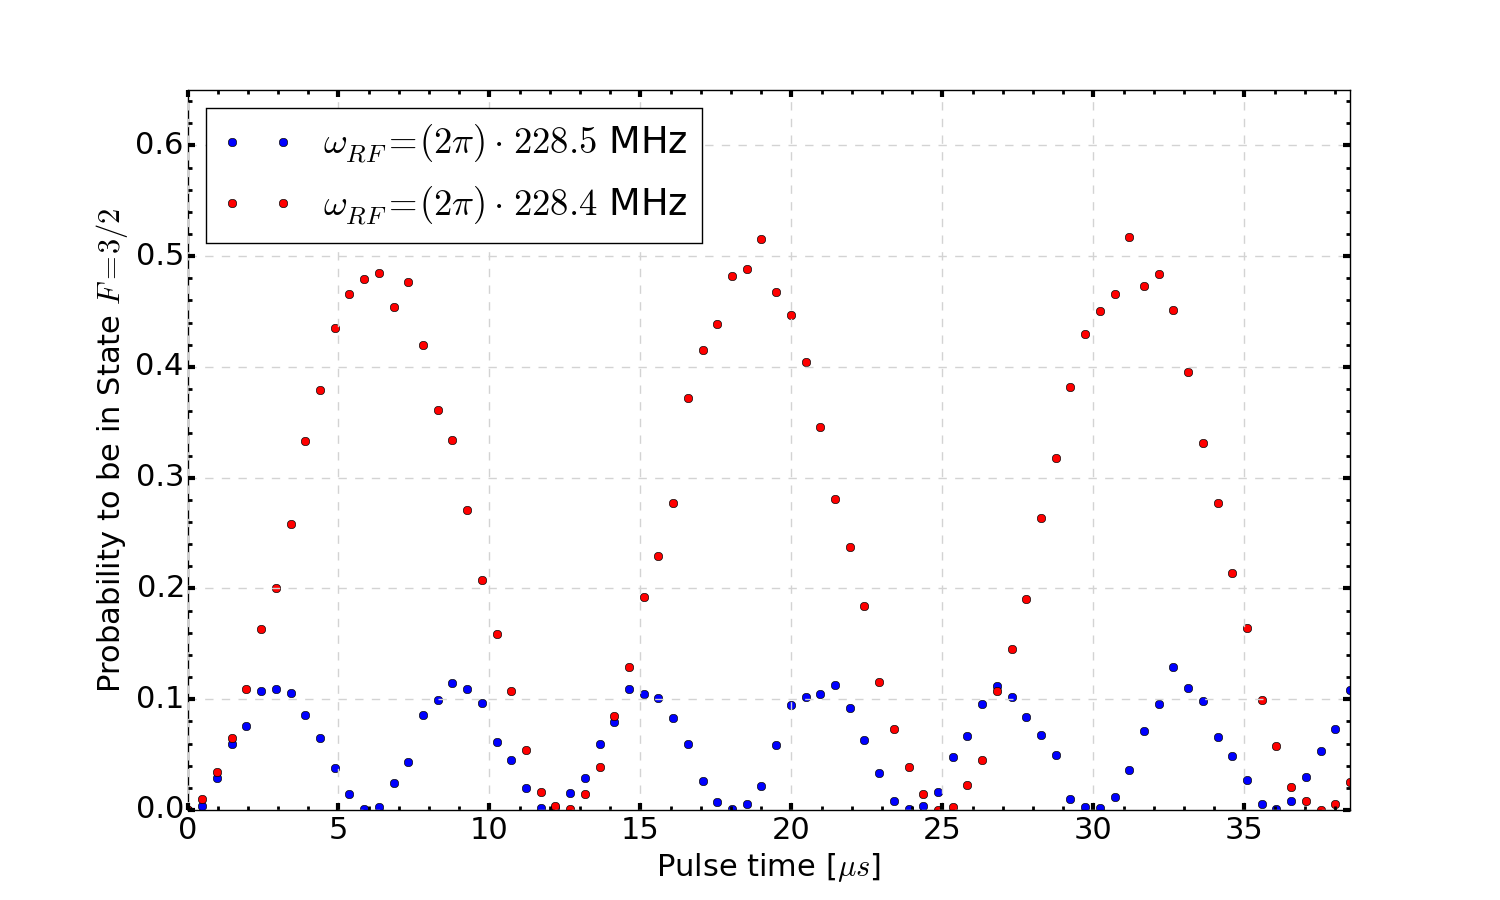
\includegraphics[angle=0, width=0.75\textwidth]
{./part1/interaction/RabiOscillations2_v3.png}
\else
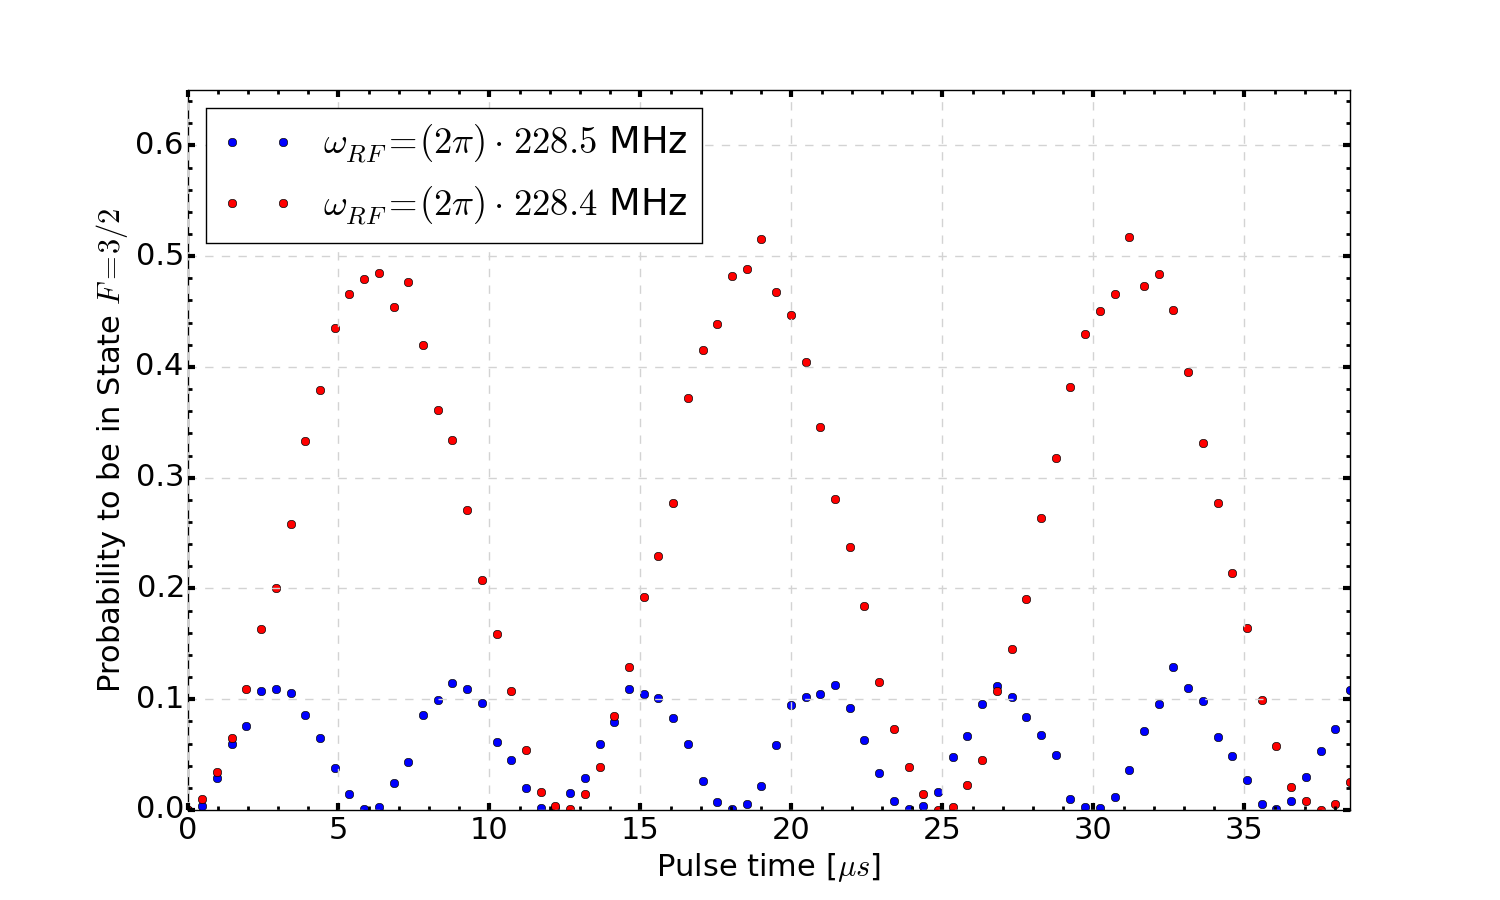
\includegraphics[angle=0, width=0.75\textwidth]
{./part1/interaction/RabiOscillations2_v3.eps}
\fi

\caption{Вы хотите измерить частоту перехода $f_0 = \frac{\omega_o}{2
  \pi}$ между двумя состояниями атома лития посредством оценки
  осцилляций Раби. Вы приготавливаете холодное облако атомов лития в
  состоянии $\left|1\right>$ (так называемое $\left|F=1/2\right>$
  состояние) и вы можете применять электромагнитный импульс
  фиксированной интенсивности и изменяемой длительности
  $\tau$. Окончательно вы измеряете число атомов в состоянии
  $\left|2\right>$ (так называемое $\left|F=3/2\right>$
  состояние).
  Вы знаете, что разность частот между этими двумя уровнями близка к
  $2 \pi \cdot 228.5 \mbox{МГц}$, следовательно вы применяете
  электромагнитный импульс с частотой близкой к этой величине, вначале
  с частотой $\omega_1 = 2 \pi \cdot 228.5 \mbox{МГц}$, потом вы повторяете
  измерения с частотой $\omega_1 = 2 \pi \cdot 228.4 \mbox{МГц}$. Результат
  изображен на представленном рисунке. Какова
  частота перехода $f_0 = \frac{\omega_o}{2 \pi}$ между двумя
  состояниями атома лития?}
\label{figPart1InteractionQuestionFreq}
\end{figure}
